\documentclass[unicode,11pt,a4paper,oneside,numbers=endperiod,openany]{scrartcl}

\renewcommand{\thesubsection}{\arabic{subsection}}

\usepackage{ifthen}
\usepackage[utf8]{inputenc}
\usepackage{graphics}
\usepackage{graphicx}
\usepackage{hyperref}
\usepackage{amsmath}

\pagestyle{plain}
\voffset -5mm
\oddsidemargin  0mm
\evensidemargin -11mm
\marginparwidth 2cm
\marginparsep 0pt
\topmargin 0mm
\headheight 0pt
\headsep 0pt
\topskip 0pt        
\textheight 255mm
\textwidth 165mm

\newcommand{\duedate} {}
\newcommand{\setduedate}[1]{%
\renewcommand\duedate {Due date:~ #1}}
\newcommand\isassignment {false}
\newcommand{\setassignment}{\renewcommand\isassignment {true}}
\newcommand{\ifassignment}[1]{\ifthenelse{\boolean{\isassignment}}{#1}{}}
\newcommand{\ifnotassignment}[1]{\ifthenelse{\boolean{\isassignment}}{}{#1}}

\newcommand{\assignmentpolicy}{
\begin{table}[h]
\begin{center}
\scalebox{0.8} {%
\begin{tabular}{|p{0.02cm}p{16cm}|}
\hline
&\\
\multicolumn{2}{|c|}{\Large\textbf{Numerical Computing 2022 ---  Submission Instructions}}\\
\multicolumn{2}{|c|}{\large\textbf{(Please, notice that following instructions are mandatory: }}\\
\multicolumn{2}{|c|}{\large\textbf{submissions that don't comply with, won't be considered)}}\\
&\\
\textbullet & Assignments must be submitted to \href{https://www.icorsi.ch/course/view.php?id=14666}{iCorsi} (i.e. in electronic format).\\
\textbullet & Provide both executable package and sources (e.g. C/C++ files, Julia). 
If you are using libraries, please add them in the file. Sources must be organized in directories called:\\
\multicolumn{2}{|c|}{\textit{Project\_number\_lastname\_firstname}}\\
& and  the  file must be called:\\
\multicolumn{2}{|c|}{\textit{project\_number\_lastname\_firstname.zip}}\\
\multicolumn{2}{|c|}{\textit{project\_number\_lastname\_firstname.pdf}}\\
\textbullet &  The TAs will grade your project by reviewing your project write-up, and looking at the implementation you attempted, and benchmarking your code's performance.\\

\textbullet & You are allowed to discuss all questions with anyone you like; however: (i) your submission must list anyone you discussed problems with and (ii) you must write up your submission independently.\\
\hline
\end{tabular}
}
\end{center}
\end{table}
}
\newcommand{\punkte}[1]{\hspace{1ex}\emph{\mdseries\hfill(#1~\ifcase#1{Points}\or{Points}\else{Points}\fi)}}


\newcommand\serieheader[6]{
\thispagestyle{empty}%
\begin{flushleft}

\includegraphics[width=0.45\textwidth]{CI_logo}
\end{flushleft}
  \noindent%
  {\large\ignorespaces{\textbf{#1}}\hspace{\fill}\ignorespaces{ \textbf{#2}}}\\ \\%
  {\large\ignorespaces #3 \hspace{\fill}\ignorespaces #4}\\
  \noindent%
  \bigskip
  \hrule\par\bigskip\noindent%
  \bigskip {\ignorespaces {\Large{\textbf{#5}}}
  \hspace{\fill}\ignorespaces \large \ifthenelse{\boolean{\isassignment}}{\duedate}{#6}}
  \hrule\par\bigskip\noindent%  \linebreak
 }

\makeatletter
\def\enumerateMod{\ifnum \@enumdepth >3 \@toodeep\else
      \advance\@enumdepth \@ne
      \edef\@enumctr{enum\romannumeral\the\@enumdepth}\list
      {\csname label\@enumctr\endcsname}{\usecounter
        {\@enumctr}%%%? the following differs from "enumerate"
	\topsep0pt%
	\partopsep0pt%
	\itemsep0pt%
	\def\makelabel##1{\hss\llap{##1}}}\fi}
\let\endenumerateMod =\endlist
\makeatother




\usepackage{textcomp}

\begin{document}


\setassignment
\setduedate{Wednesday, 12 October 2022, 23:59 AM}

\serieheader{Numerical Computing}{2022}{Student: FULL NAME}{Discussed with: FULL NAME}{Solution for Project 1}{}
\newline

\assignmentpolicy
The purpose of this assignment\footnote{This document is originally based on a SIAM book chapter from \textsl{Numerical Computing with Matlab} from  Clever B. Moler.} is to learn the importance of numerical linear algebra algorithms to solve fundamental  linear algebra problems that occur in search engines.



\section*{PageRank Algorithm }

\subsection{Theory [20 points]}

\begin{enumerate}
\item[(a)] \textbf{What are an eigenvector, an eigenvalue and an eigenbasis?}\\
An eigenvector is a nonzero vector that, when involved in a linear transformation gets stretched and scaled but stays on the same span. \\\\
An eigenvalue, denoted with symbol $\lambda$ represents the factor of how much the eigenvector gets stretched along his direction. \\
The eigenvalue can be negative, as it means the resulting vectors inverts its direction after the linear transformation.  \\\\
An eigenbasis is a diagonal matrix that has eigenvectors as its columns, and eigenvalues along its diagonal.\\
Given a matrix $A$ and a linear transformation $T$, 
if there exists a vector $v$ such that $Tv = \lambda v$,
then $v$ is an eigenvector of $A$ and $\lambda$ is an eigenvalue of A.
If there exists a set of vectors $V$ such that $T(V) = \lambda V$, then $V$ is an eigenbasis of $A$.

% An eigenvector is a vector that doesn't change direction when a linear transformation is applied to it.
% An eigenvalue is a scalar that is multiplied by the eigenvector.
% An eigenbasis is a set of eigenvectors that are linearly independent.

% Given a matrix $A$ and a linear transformation $T$, 
% if there exists a vector $v$ such that $Tv = \lambda v$,
% then $v$ is an eigenvector of $A$ and $\lambda$ is an eigenvalue of A.
% If there exists a set of vectors $V$ such that $T(V) = \lambda V$, then $V$ is an eigenbasis of $A$.


\item[(b)] \textbf{What assumptions should be made to guarantee convergence of the power method?}\\
We need to assume that the eigenvalue to which the power method converges 
is the dominant eigenvalue, and we also need to assume that the randomly-chosen initial vector has a component in the same direction as the eigenvector.\\
Also, to guarantee a faster convergence, $\lambda _1$ and $\lambda _2$ have to be distant, as the asymptotic error constant is $|\frac{\lambda _1}{\lambda _2}|$ meaning convergence is extremely slow if the two eigenvalues are close to each other.

\item[(c)] \textbf{What is the shift and invert approach?}\\
As mentioned previously, if the eigenvalues are close to each other convergence can be extremely slow.\\
The inverse iteration uses the shift and invert tecnique to speed up the convergence.

If the eigenvalues of $A$ are $\lambda_j$, the eigenvalues of $A -\alpha I$ are $\lambda_j - \alpha$, 
and the eigenvalues of $B = (A-\alpha I)^{-1}$ are $\mu_j = \frac{1}{\lambda_j - \alpha}$

If we apply the power method to $B$ we get an improve rate of $|\frac{\mu_2}{\mu_1}| = |\frac{\frac{1}{\lambda_2 - \alpha}}{\frac{1}{\lambda_1 - \alpha}}| = |\frac{\lambda_1 - \alpha}{\lambda_2 - \alpha}|$.\\
It is therefore in our best interests to find an $\alpha$ as close as possible to any eigenvalue.\\
The shift and invert approach is to choose $\alpha$ such that the improve rate is as small as possible.


\item[(d)] \textbf{What is the difference in cost of a single iteration of the power method, compared to the inverse iteration?}\\
Using the power method, each iteration involves a \textit{matrix-vector multiplication}, while the \textit{inverse iteration} requires solving a linear system.
Solving a linear system is way more computationally expensive than a matrix-vector multiplication, having a fast convergence for inverse iteration is necessary in order for it to to be effective; 
this would be impossible when tackling larger issues such as Internet searching.
Inverse iteration must be used for smaller problems or problems with special structure that enables fast direct methods.


\item[(e)] \textbf{What is a Rayleigh quotient and how can it be used for eigenvalue computations?}\\
The Rayleigh quotient is an improvement over the inverse iteration method for finding eigenvalues.\\
It guarantees very fast convergence, in most cases even cubically. To guarantee fast convergence, we change the value of $\alpha$ dynamically to be the Rayleigh quotient in each iteration.\\
Even though Rayleigh quotient iteration is more computationally expensive as it requires to refactor the matrix in each iteration, the cubic convergence makes it worthwhile.

\end{enumerate}

\newpage
\subsection{Other webgraphs [10 points]}
In this part of the assignment, the pageranks of three different subsets of the Web (Chess.com, RSI, and StackOverflow) has been computed.
In each section we show the connectivity graph of the webgraph, the pagerank graph and the top 10 pages with the highest pagerank.

The experiments are all done by calling the same function \texttt{surfer} that access the desired homepage and then generates a 500-by-500 test case.


\subsubsection{Webgraph 1: Chess.com}
\begin{figure}[h!]
    \begin{minipage}{0.5\textwidth}
        \centering
        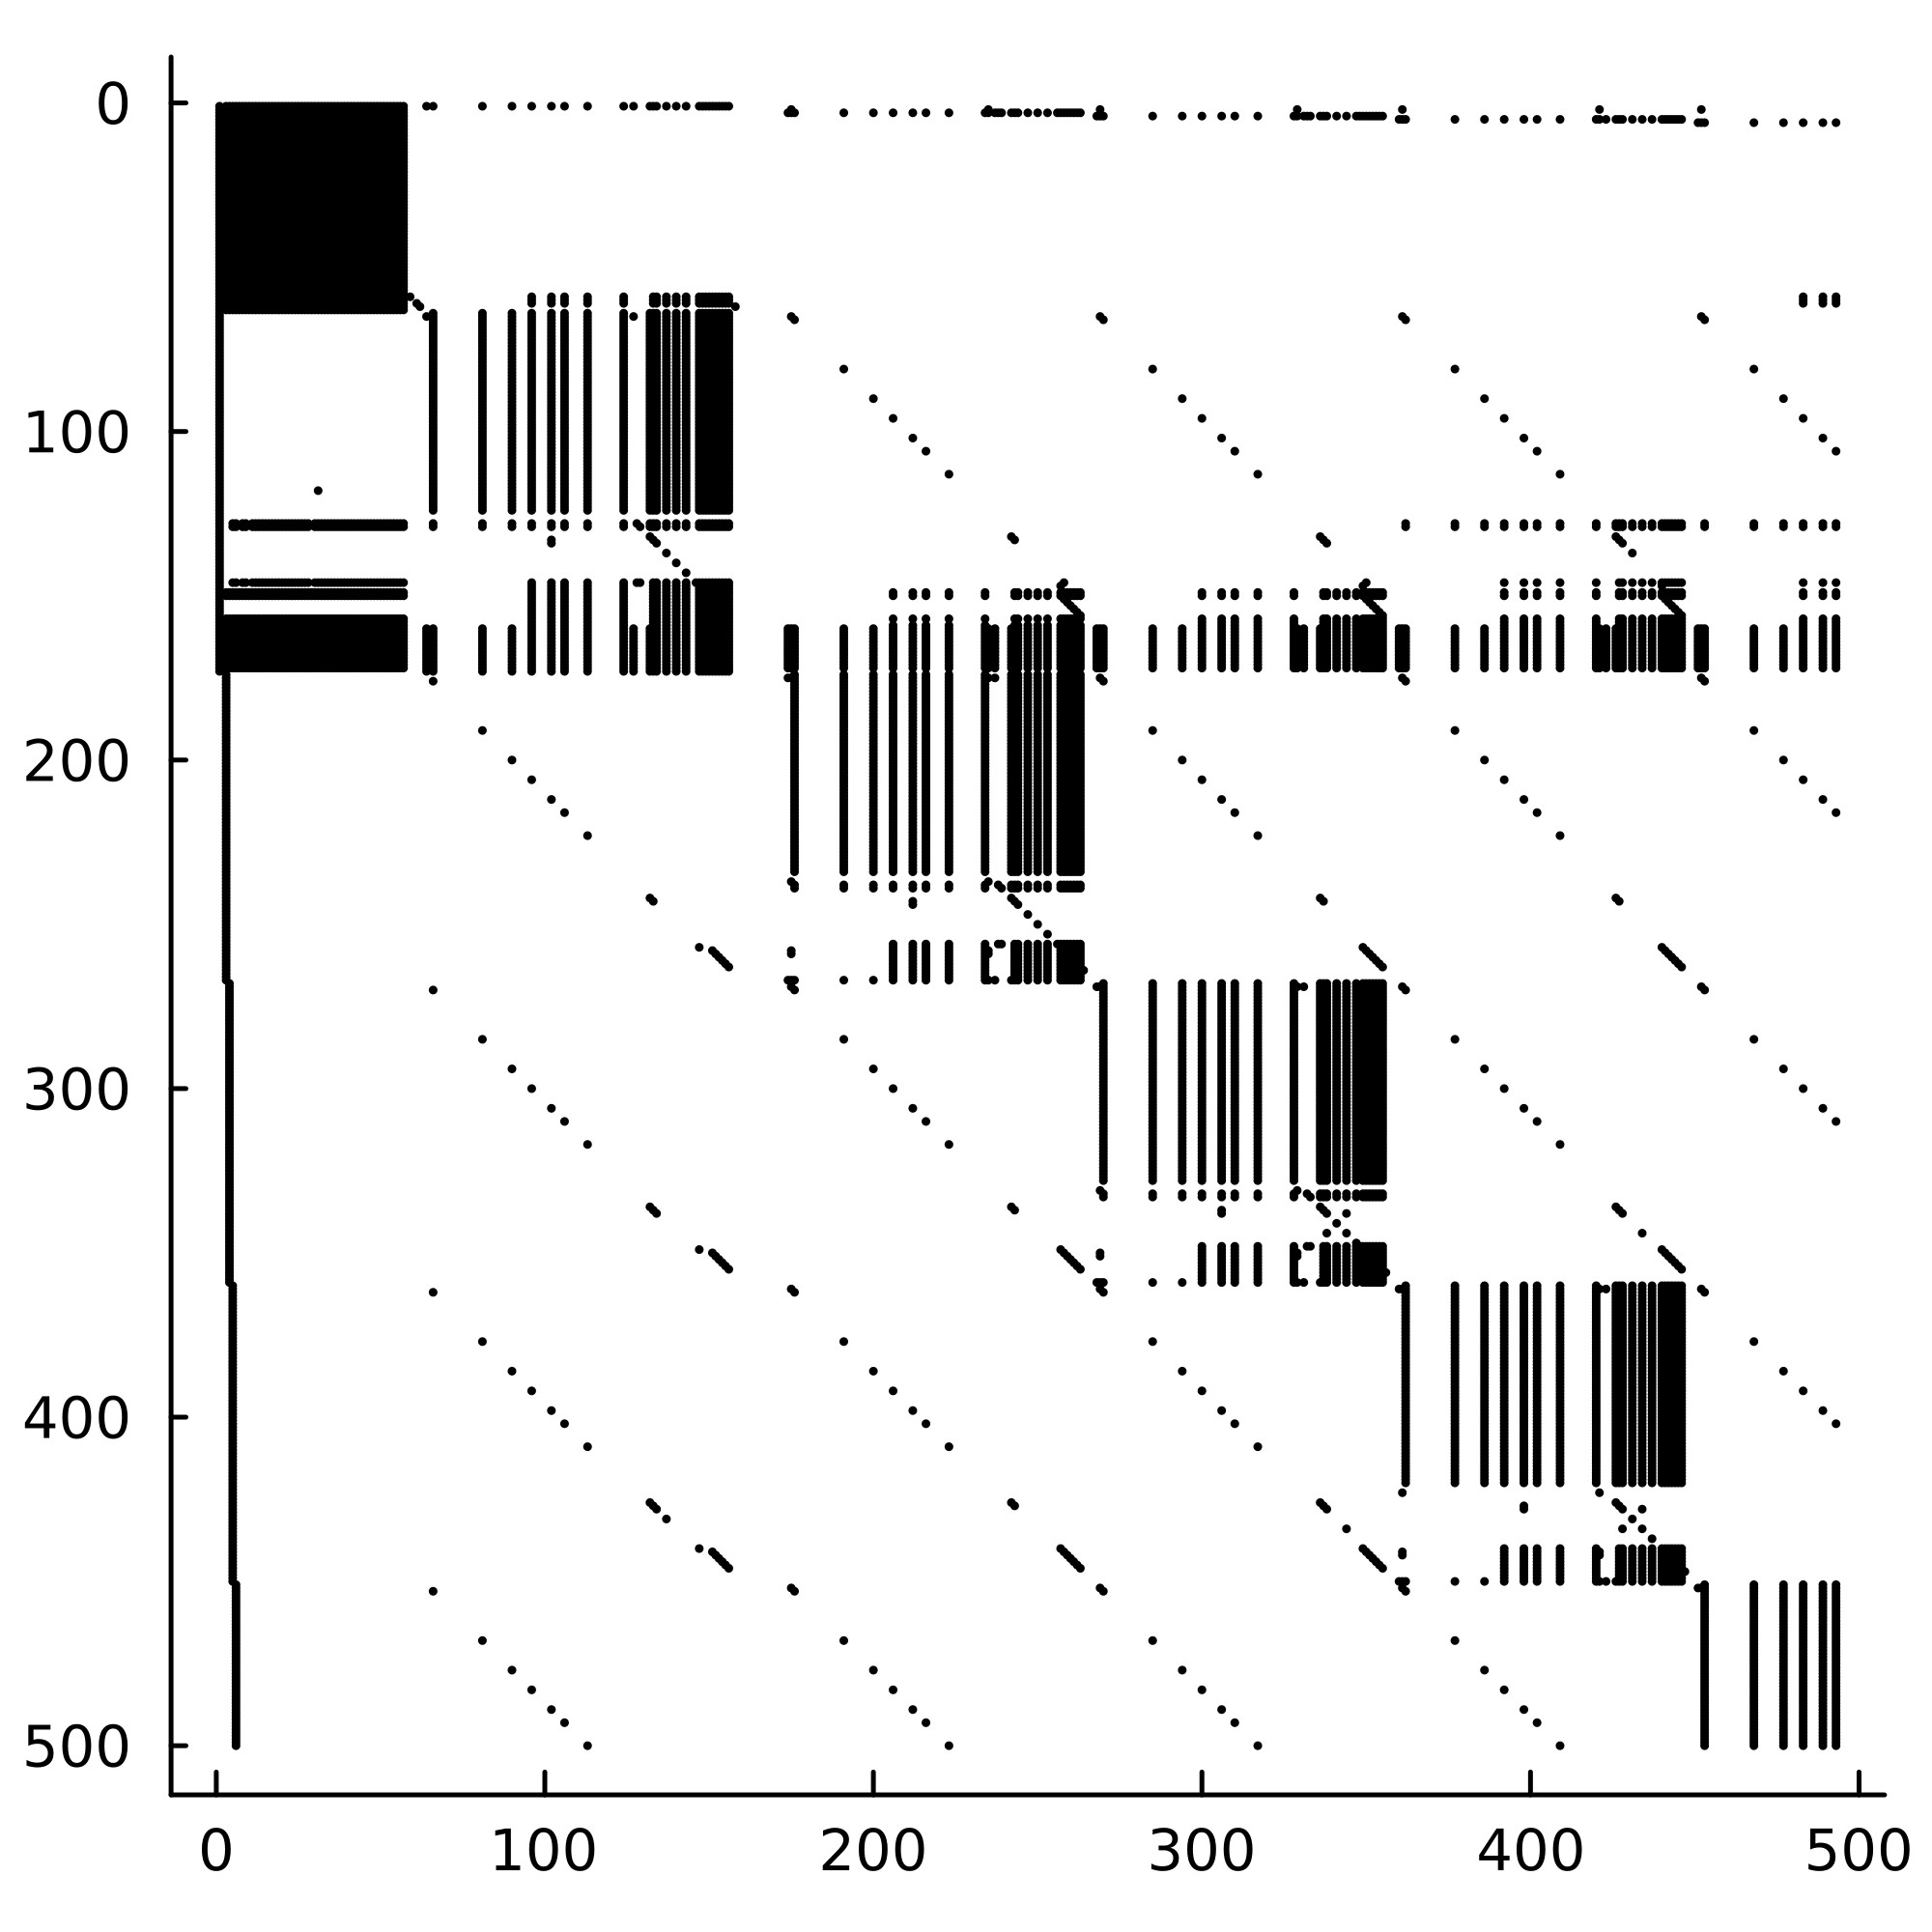
\includegraphics[height=5cm]{fig/chess.jpg}
        \caption{Spy plot of the Chess.com webgraph.}
        \label{fig:chesscom}
    \end{minipage}
    \begin{minipage}{0.5\textwidth}
        \centering
        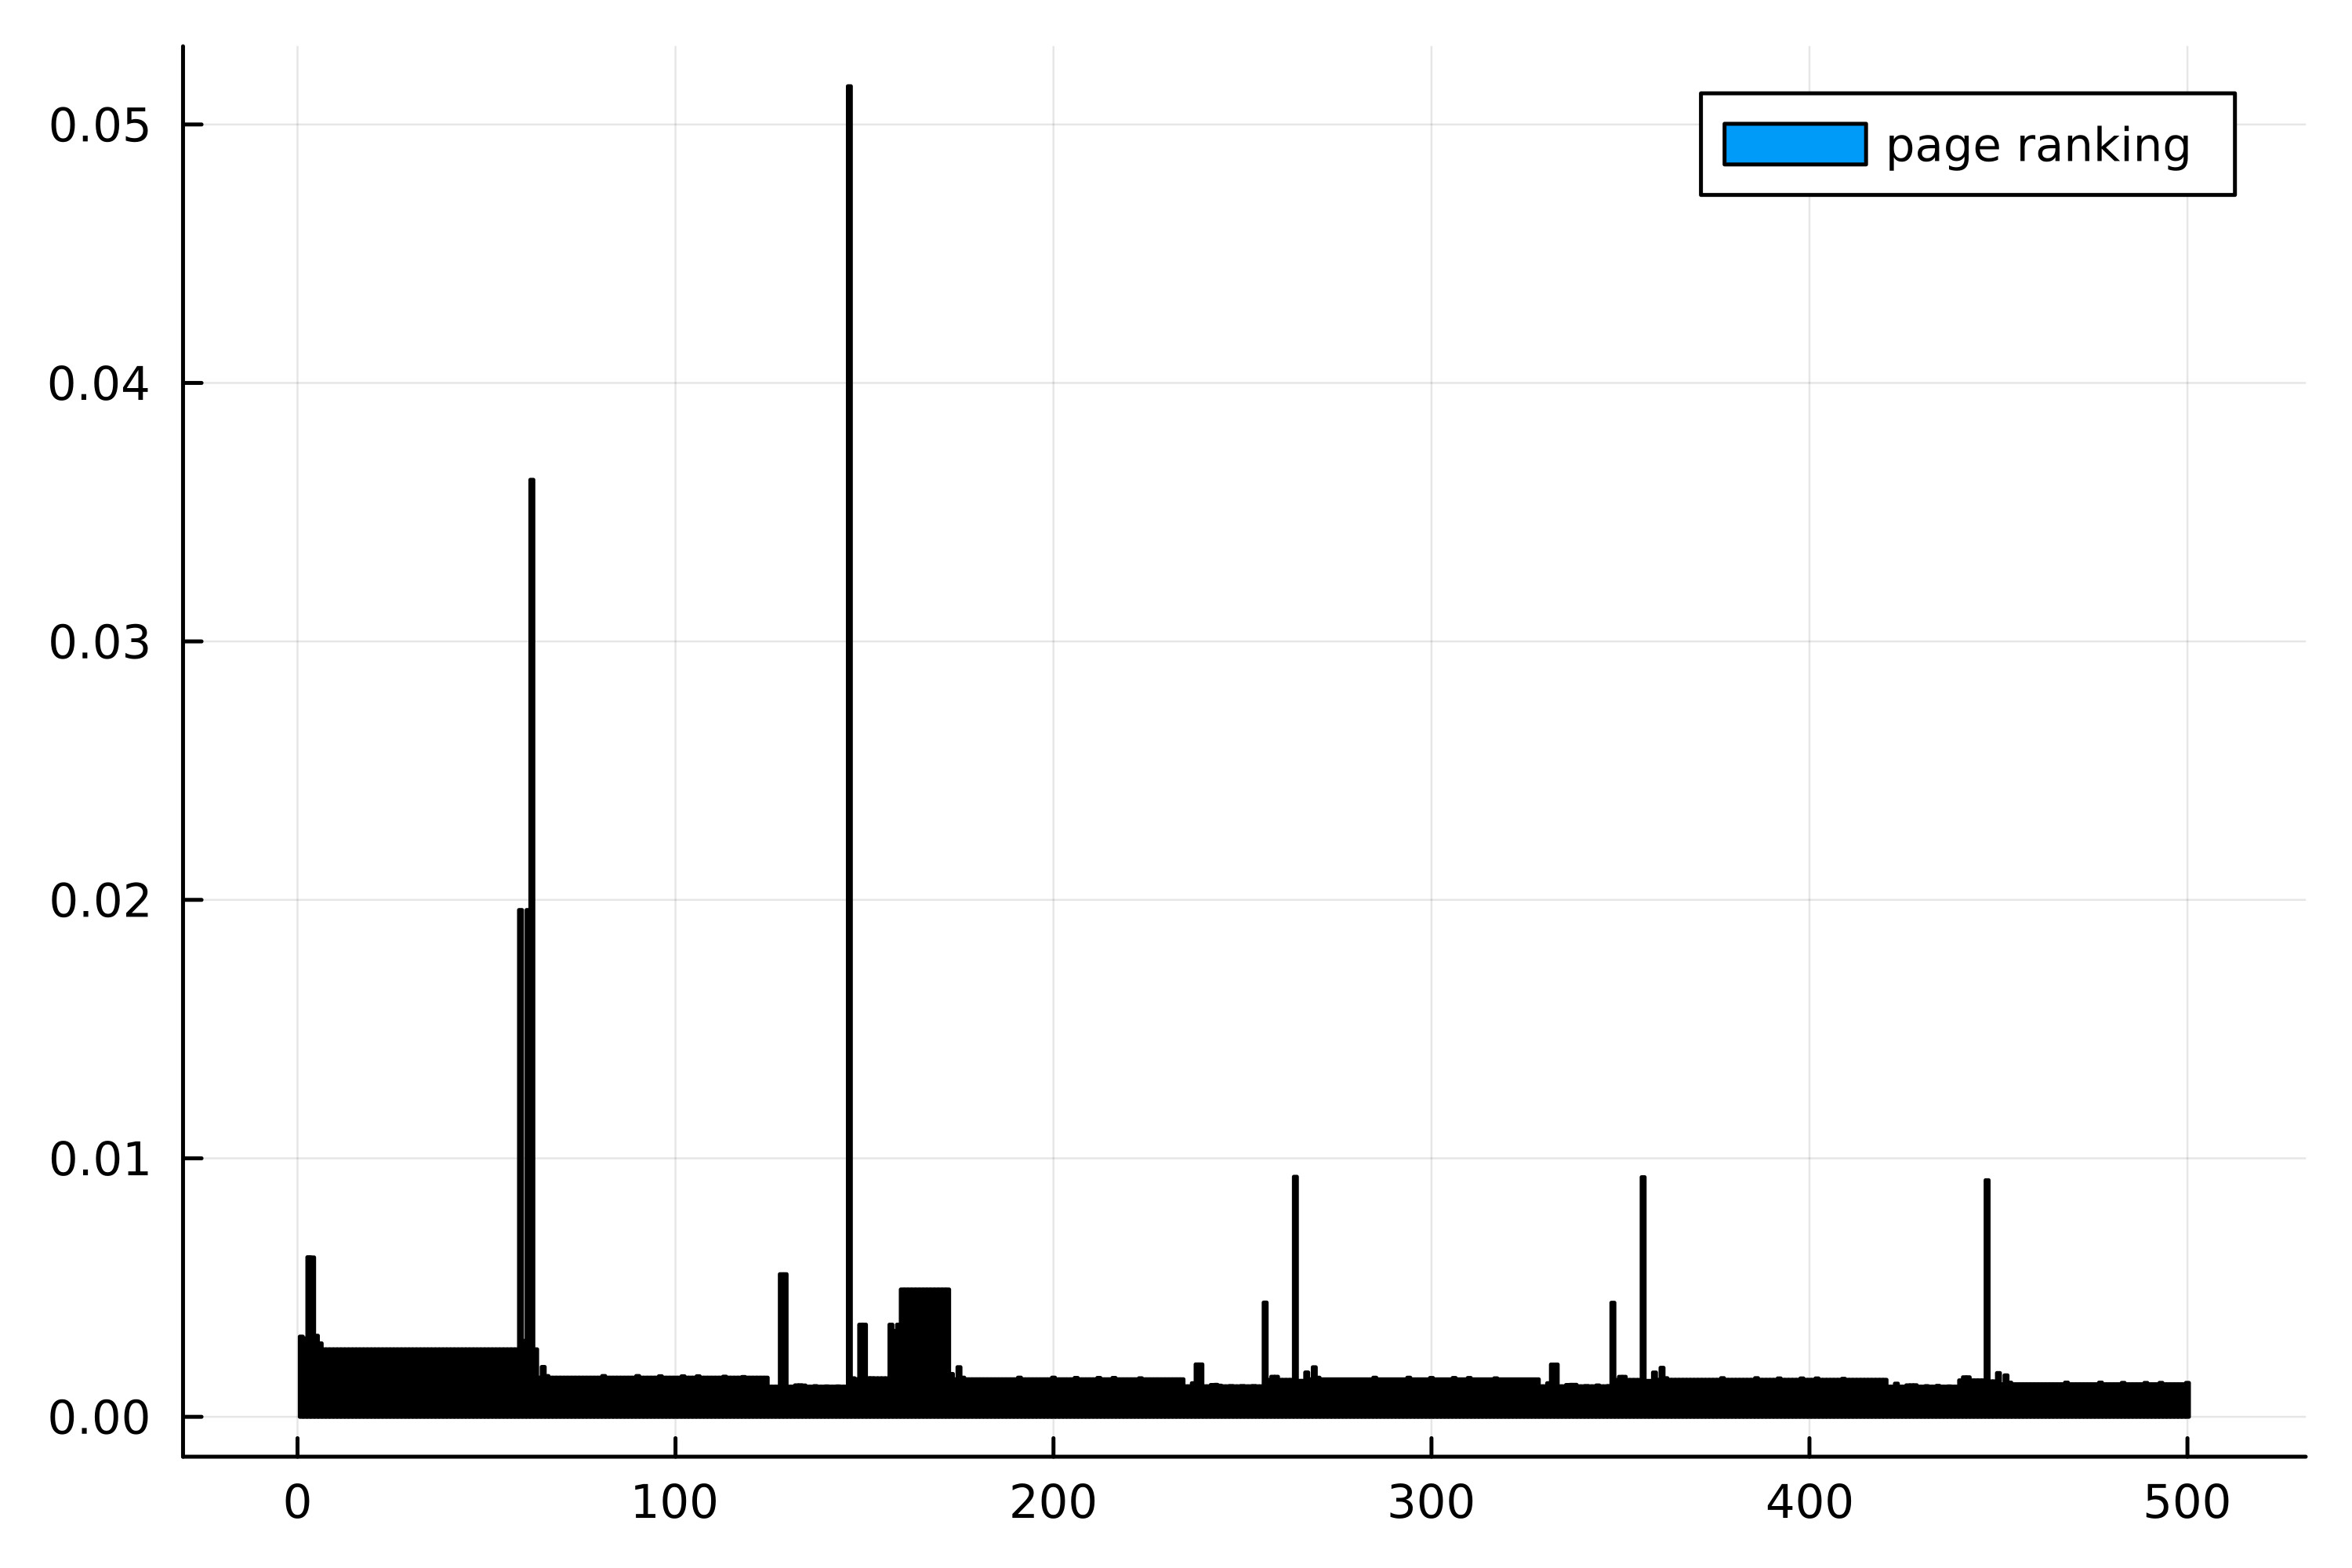
\includegraphics[height=5cm]{fig/chess_pagerank.jpg}
        \caption{PageRank of Chess.com webgraph.}
        \label{fig:chesscom_pagerank}
    \end{minipage}
\end{figure}

\begin{table}[h!]
    \small
    \centering
    \begin{tabular}{|l|l|l|l|l|} 
        \hline
        \textbf{Index} & \textbf{Page-rank} & \textbf{In} & \textbf{Out} & \textbf{Url}\\
        \hline
        146 &    0.05148 &  96 &   1 & \tiny{\url{https://support.chess.com}} \\
         62 &  0.0362528 &  58 &   1 & \tiny{\url{https://www.instagram.com/wwwchesscom/}} \\
         59 &  0.0196081 &  80 &   1 & \tiny{\url{https://twitter.com/chesscom}} \\
         61 &  0.0196081 &  80 &   1 & \tiny{\url{https://www.twitch.tv/chess}} \\
        264 & 0.00928716 &  19 &   1 & \tiny{\url{https://twitter.com/chesscom_es}} \\
        356 & 0.00927139 &  19 &   1 & \tiny{\url{https://twitter.com/chesscom_fr}} \\
        447 & 0.00915483 &  19 &   1 & \tiny{\url{https://twitter.com/chesscom_de}} \\
          3 &  0.0061748 &  84 & 174 & \tiny{\url{https://www.chess.com/es}} \\
          4 & 0.00616691 &  84 & 173 & \tiny{\url{https://www.chess.com/fr}} \\
        128 & 0.00551868 & 103 &   2 & \tiny{\url{https://support.chess.com/collection/136-community-safety}} \\
        \hline
    \end{tabular}
    \caption{The ten most important entries in the PageRank of the Chess.com webgraph.}
    \label{table:chesscom}
\end{table}



\subsubsection{Webgraph 2: Radiotelevisione svizzera di lingua italiana (RSI)}
\begin{figure}[h!]
    \begin{minipage}{0.5\textwidth}
        \centering
        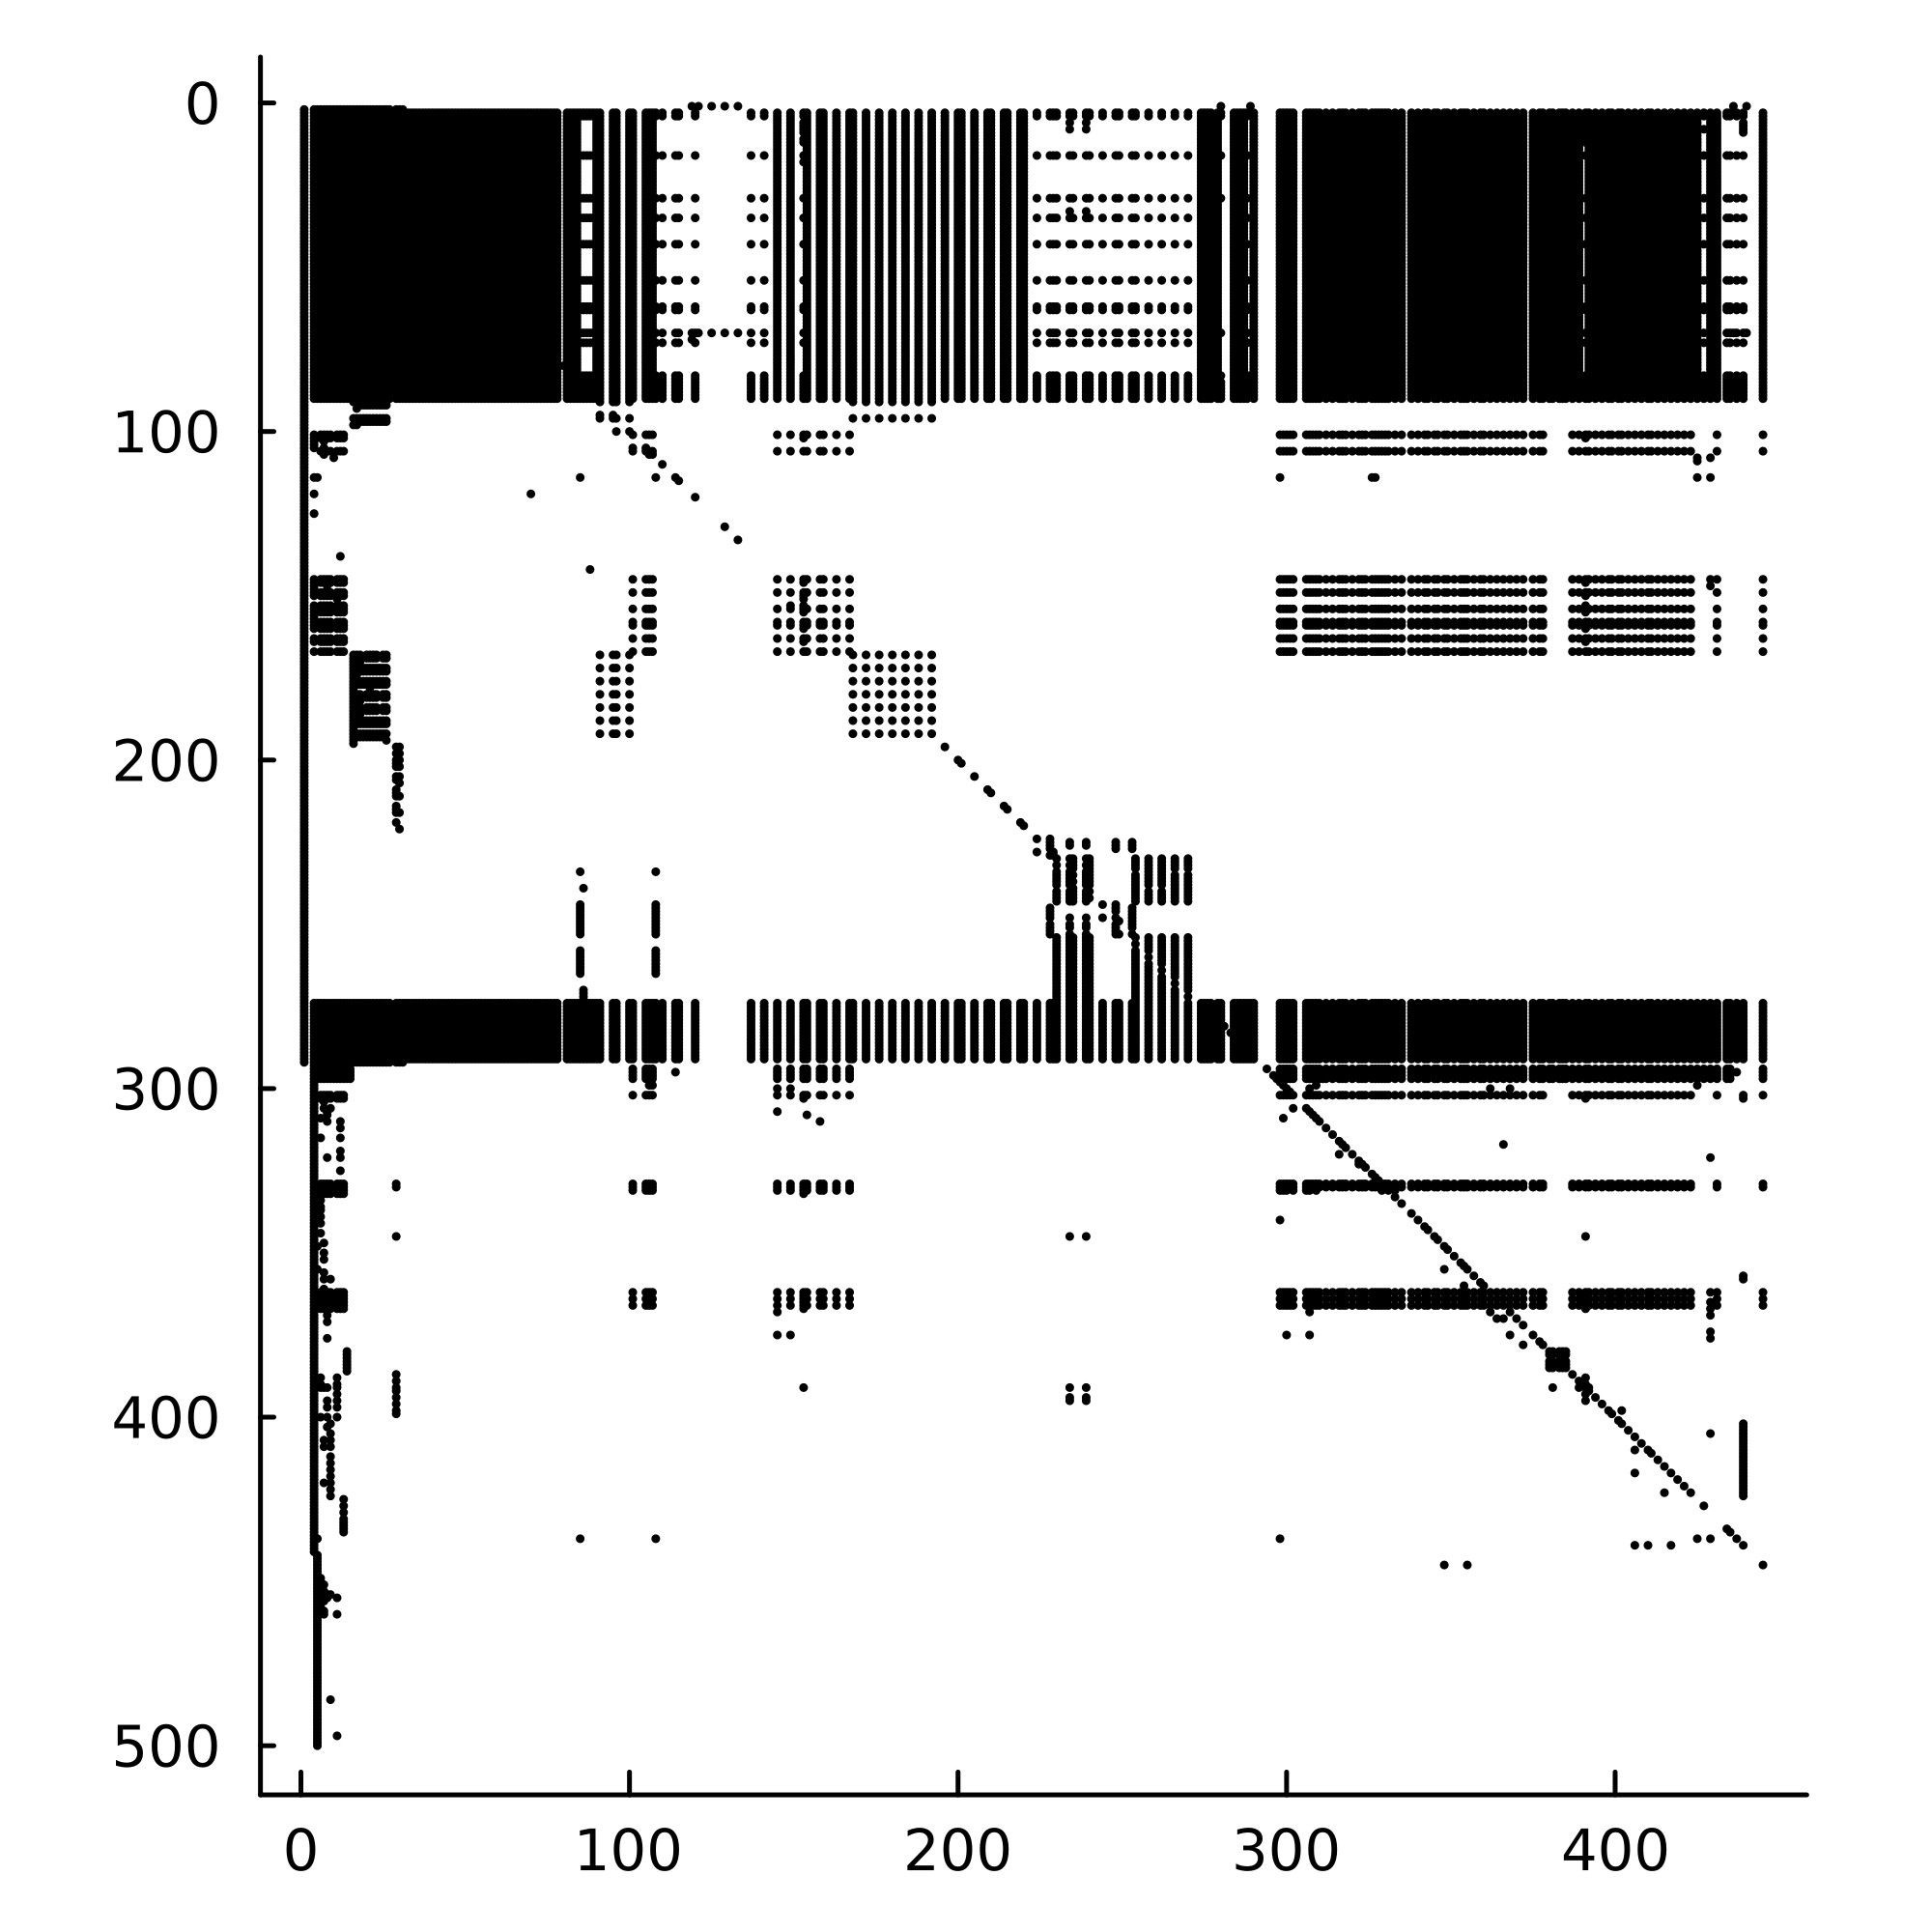
\includegraphics[height=5cm]{fig/RSI.jpg}
        \caption{Spy plot of the RSI webgraph.}
        \label{fig:RSI}
    \end{minipage}
    \begin{minipage}{0.5\textwidth}
        \centering
        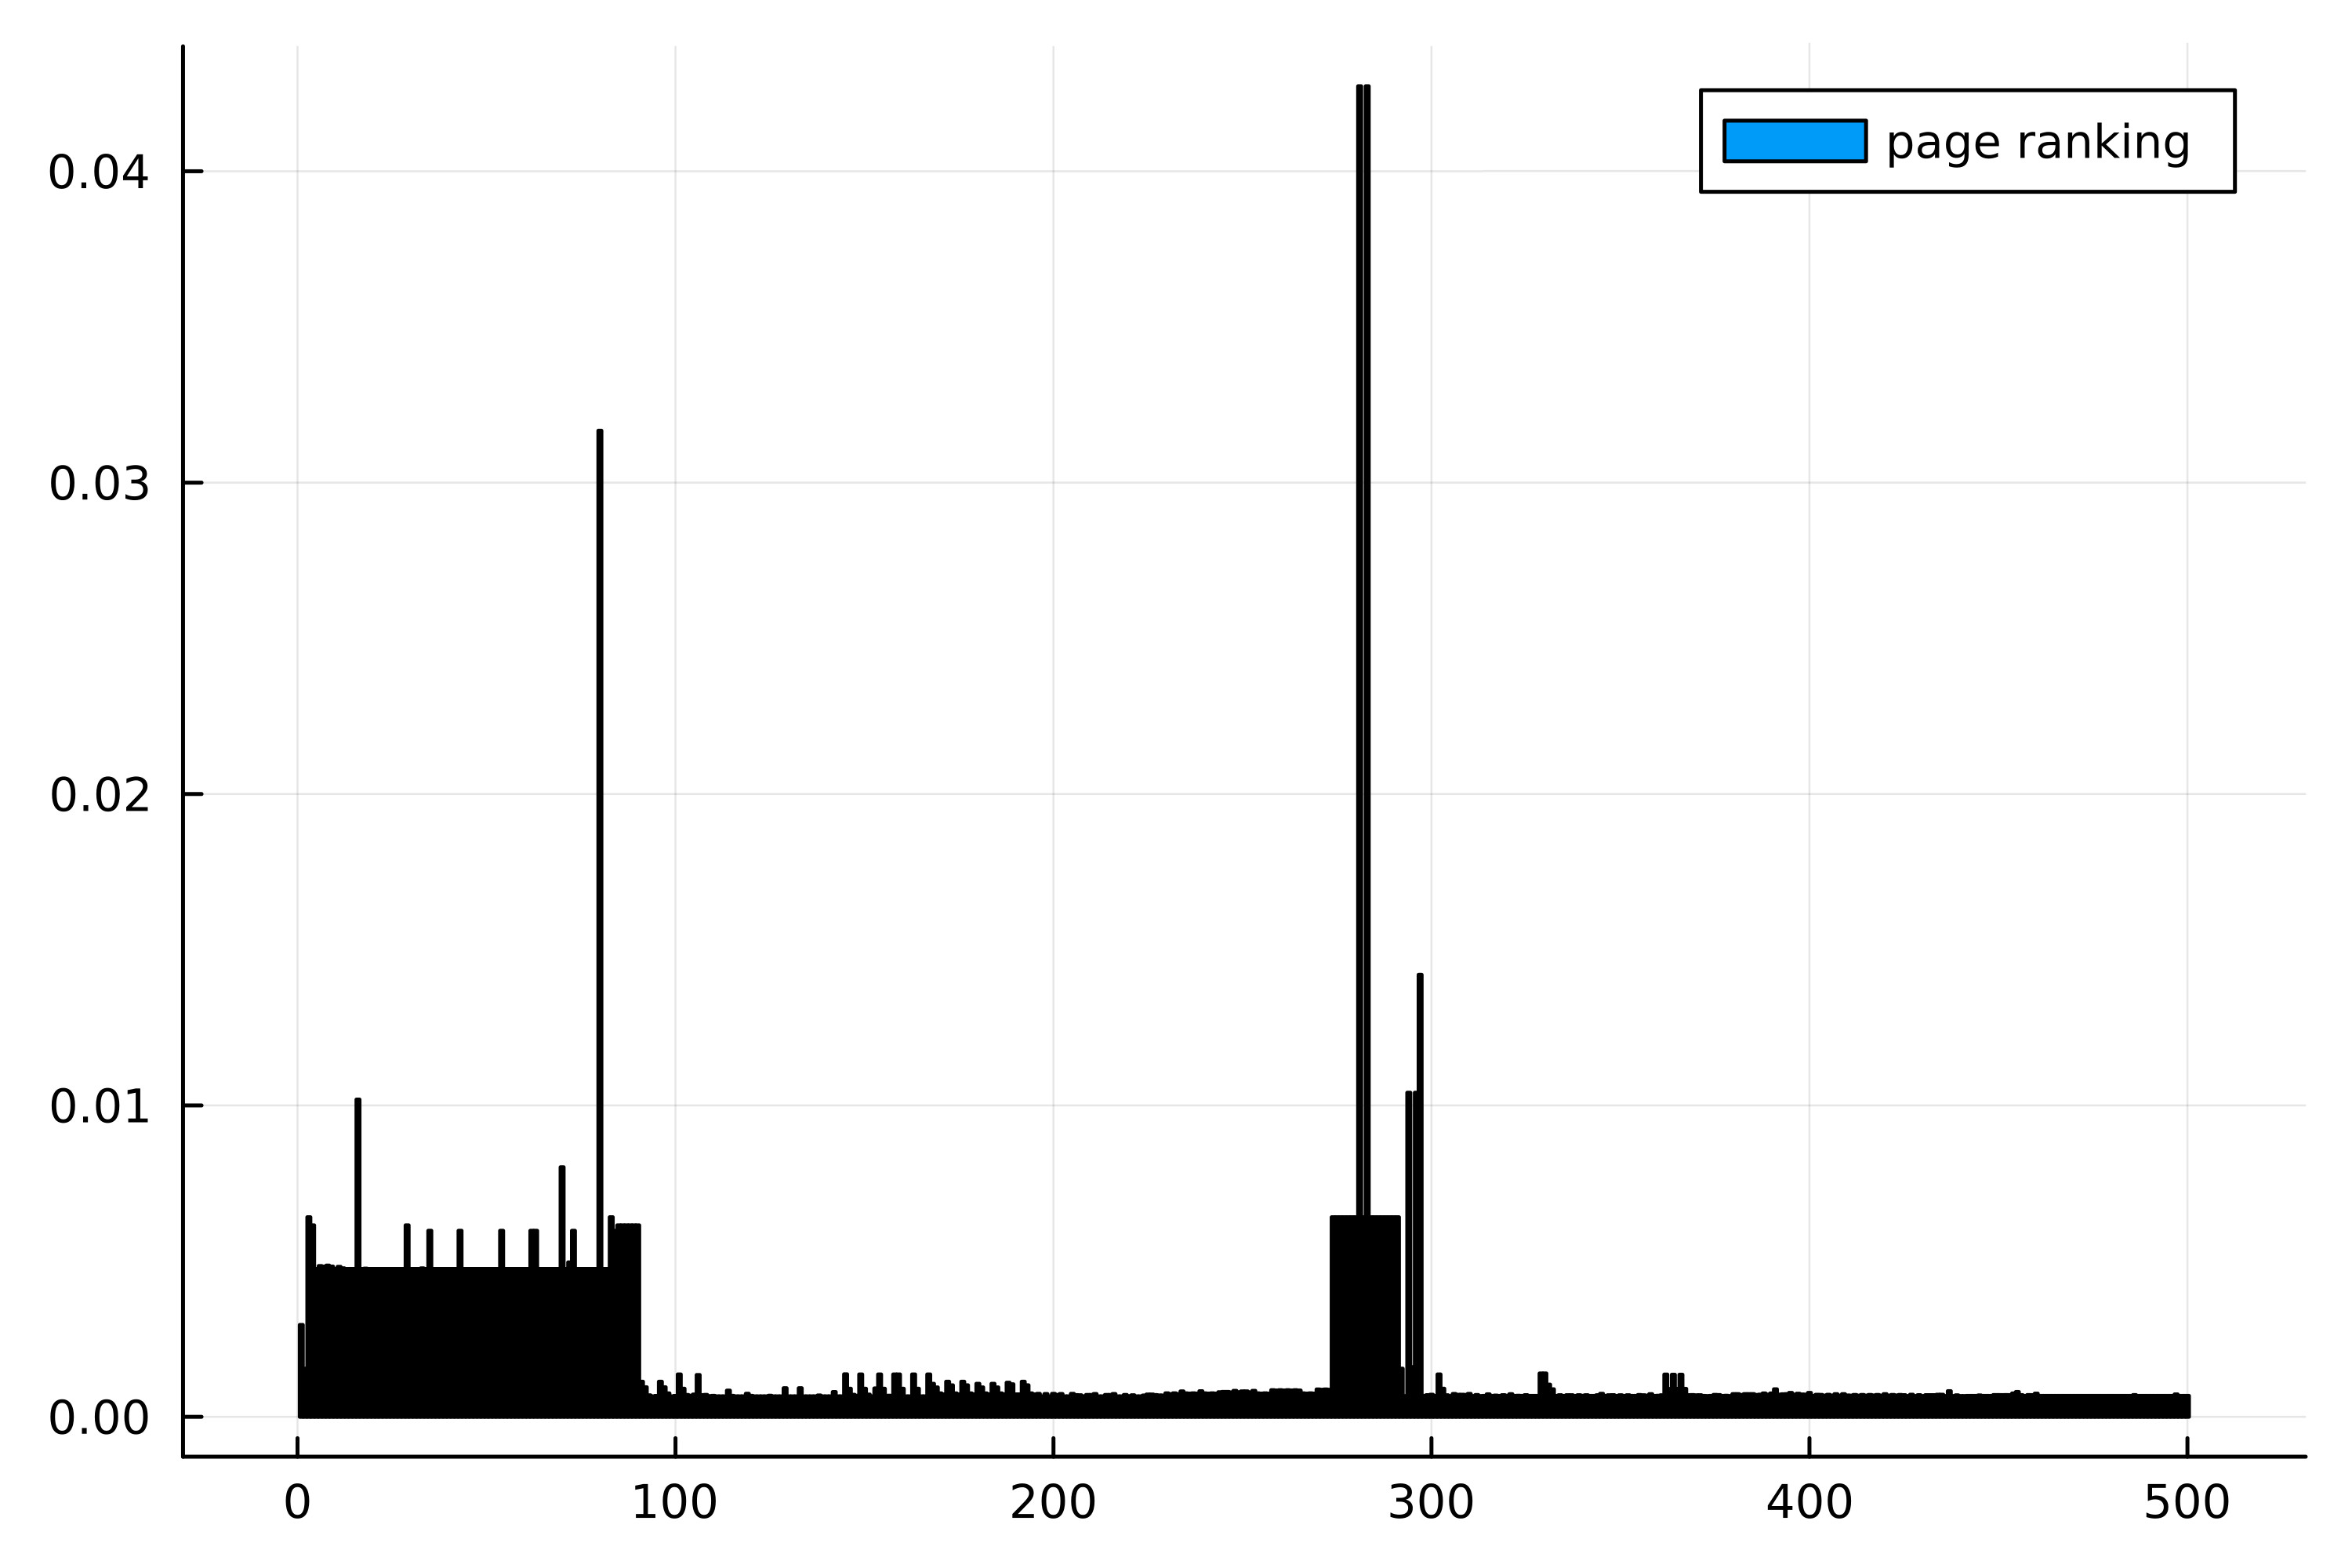
\includegraphics[height=5cm]{fig/RSI_pagerank.jpg}
        \caption{PageRank of RSI webgraph.}
        \label{fig:RSI_pagerank}
    \end{minipage}
\end{figure}

\begin{table}[h!]
    \small
    \centering
    \begin{tabular}{|l|l|l|l|l|} 
        \hline
        \textbf{Index} & \textbf{Page-rank} & \textbf{In} & \textbf{Out} & \textbf{Url}\\
        \hline
        281 &  0.0427305 & 242 &   1 & \tiny{\url{https://www.srgssr.ch/it/chi-siamo/organizzazione/piattaforma-per-segnalazioni-di-illeciti}} \\
        283 &  0.0427305 & 242 &   1 & \tiny{\url{https://www.corsi-rsi.ch/}} \\
         80 &  0.0316679 & 202 &   1 & \tiny{\url{https://boutique.rsi.ch/}} \\
        297 &  0.0141953 & 110 &   1 & \tiny{\url{https://www.instagram.com/rsinews/}} \\
        294 &  0.0104083 & 109 &   1 & \tiny{\url{https://www.youtube.com/channel/UC6UUxoC7DGUUlUHcJvulsfQ}} \\
        296 &  0.0104083 & 109 &   1 & \tiny{\url{https://twitter.com/rsinews}} \\
         16 &  0.0101878 & 241 & 139 & \tiny{\url{https://www.rsi.ch/sport/}} \\
         70 &  0.0080161 & 247 & 107 & \tiny{\url{https://www.rsi.ch/meteo/}} \\
        288 & 0.00640957 & 241 &  37 & \tiny{\url{https://www.rsi.ch/audio/}} \\
        284 & 0.00640957 & 241 & 106 & \tiny{\url{https://www.rsi.ch/la-rsi/Dichiarazione-sulla-protezione-dei-dati-10499633.html}} \\
        \hline
    \end{tabular}
    \caption{The ten most important entries in the PageRank of the RSI webgraph.}
    \label{table:RSI}
\end{table}

\subsubsection{Webgraph 3: StackOverflow}
\begin{figure}[!h]
    \begin{minipage}{0.5\textwidth}
        \centering
        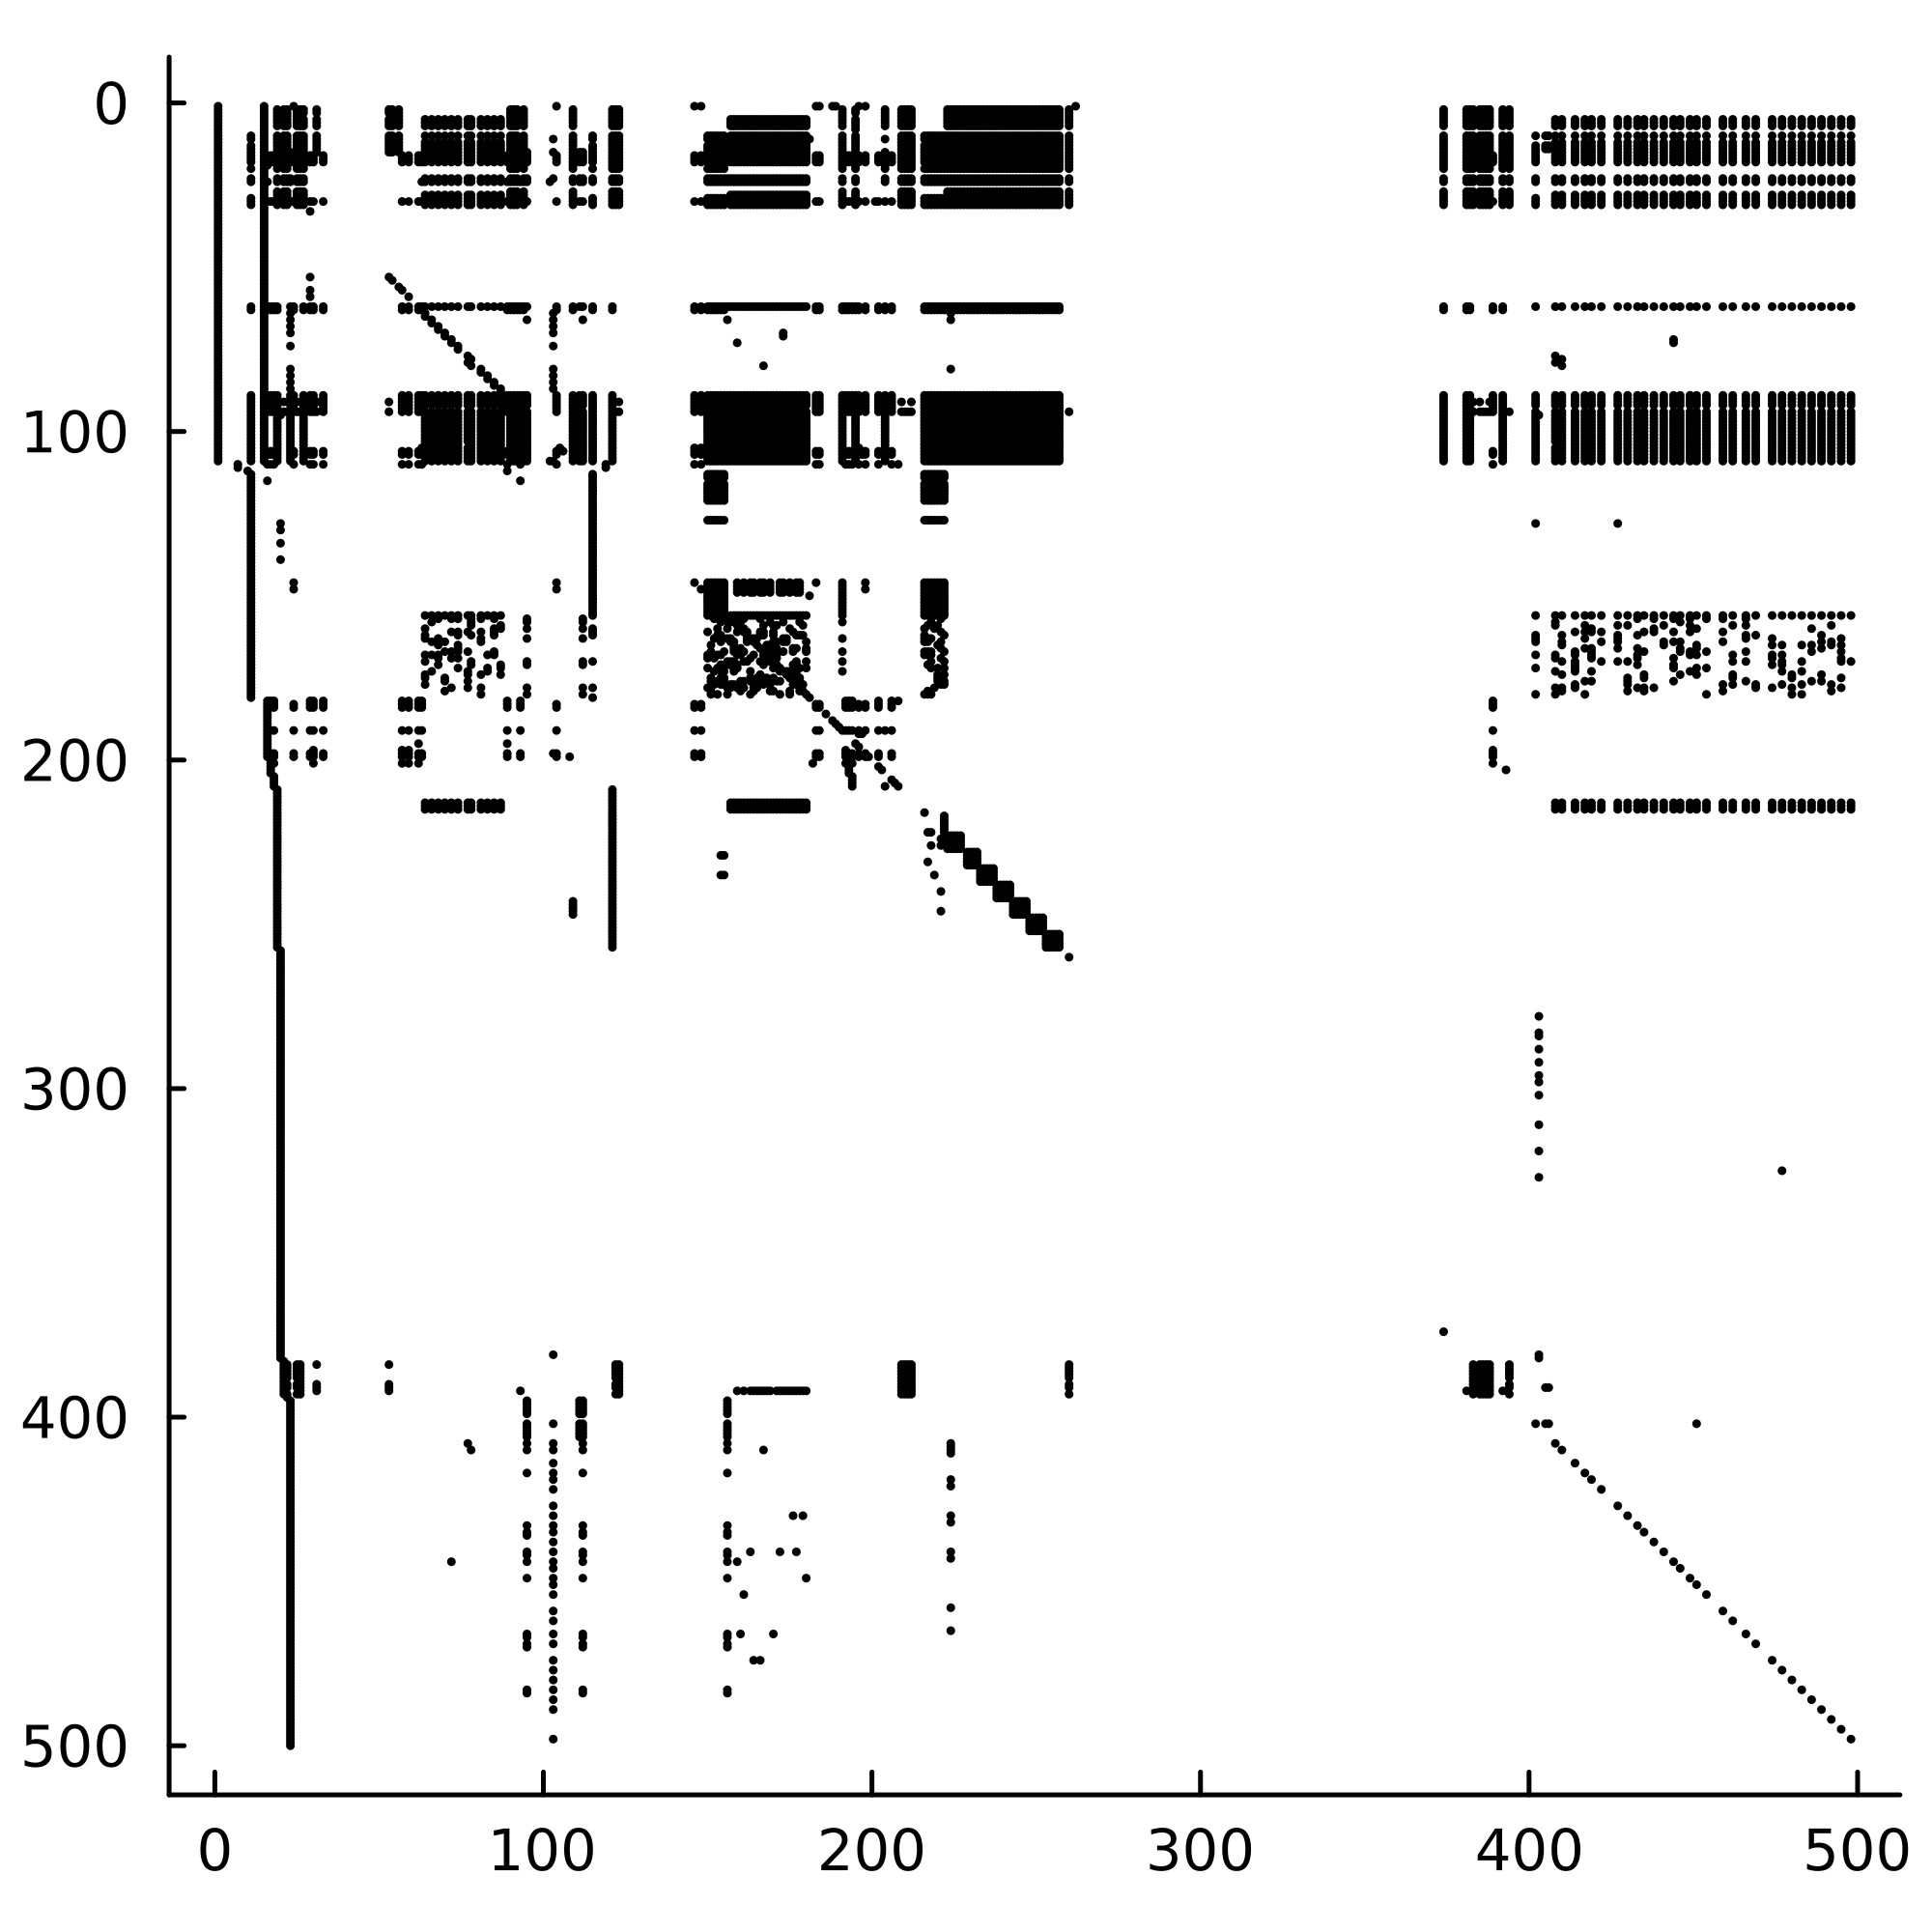
\includegraphics[height=5cm]{fig/StackOverflow.jpg}
        \caption{Spy plot of the StackOverflow webgraph.}
        \label{fig:StackOverflow}
    \end{minipage}
    \begin{minipage}{0.5\textwidth}
        \centering
        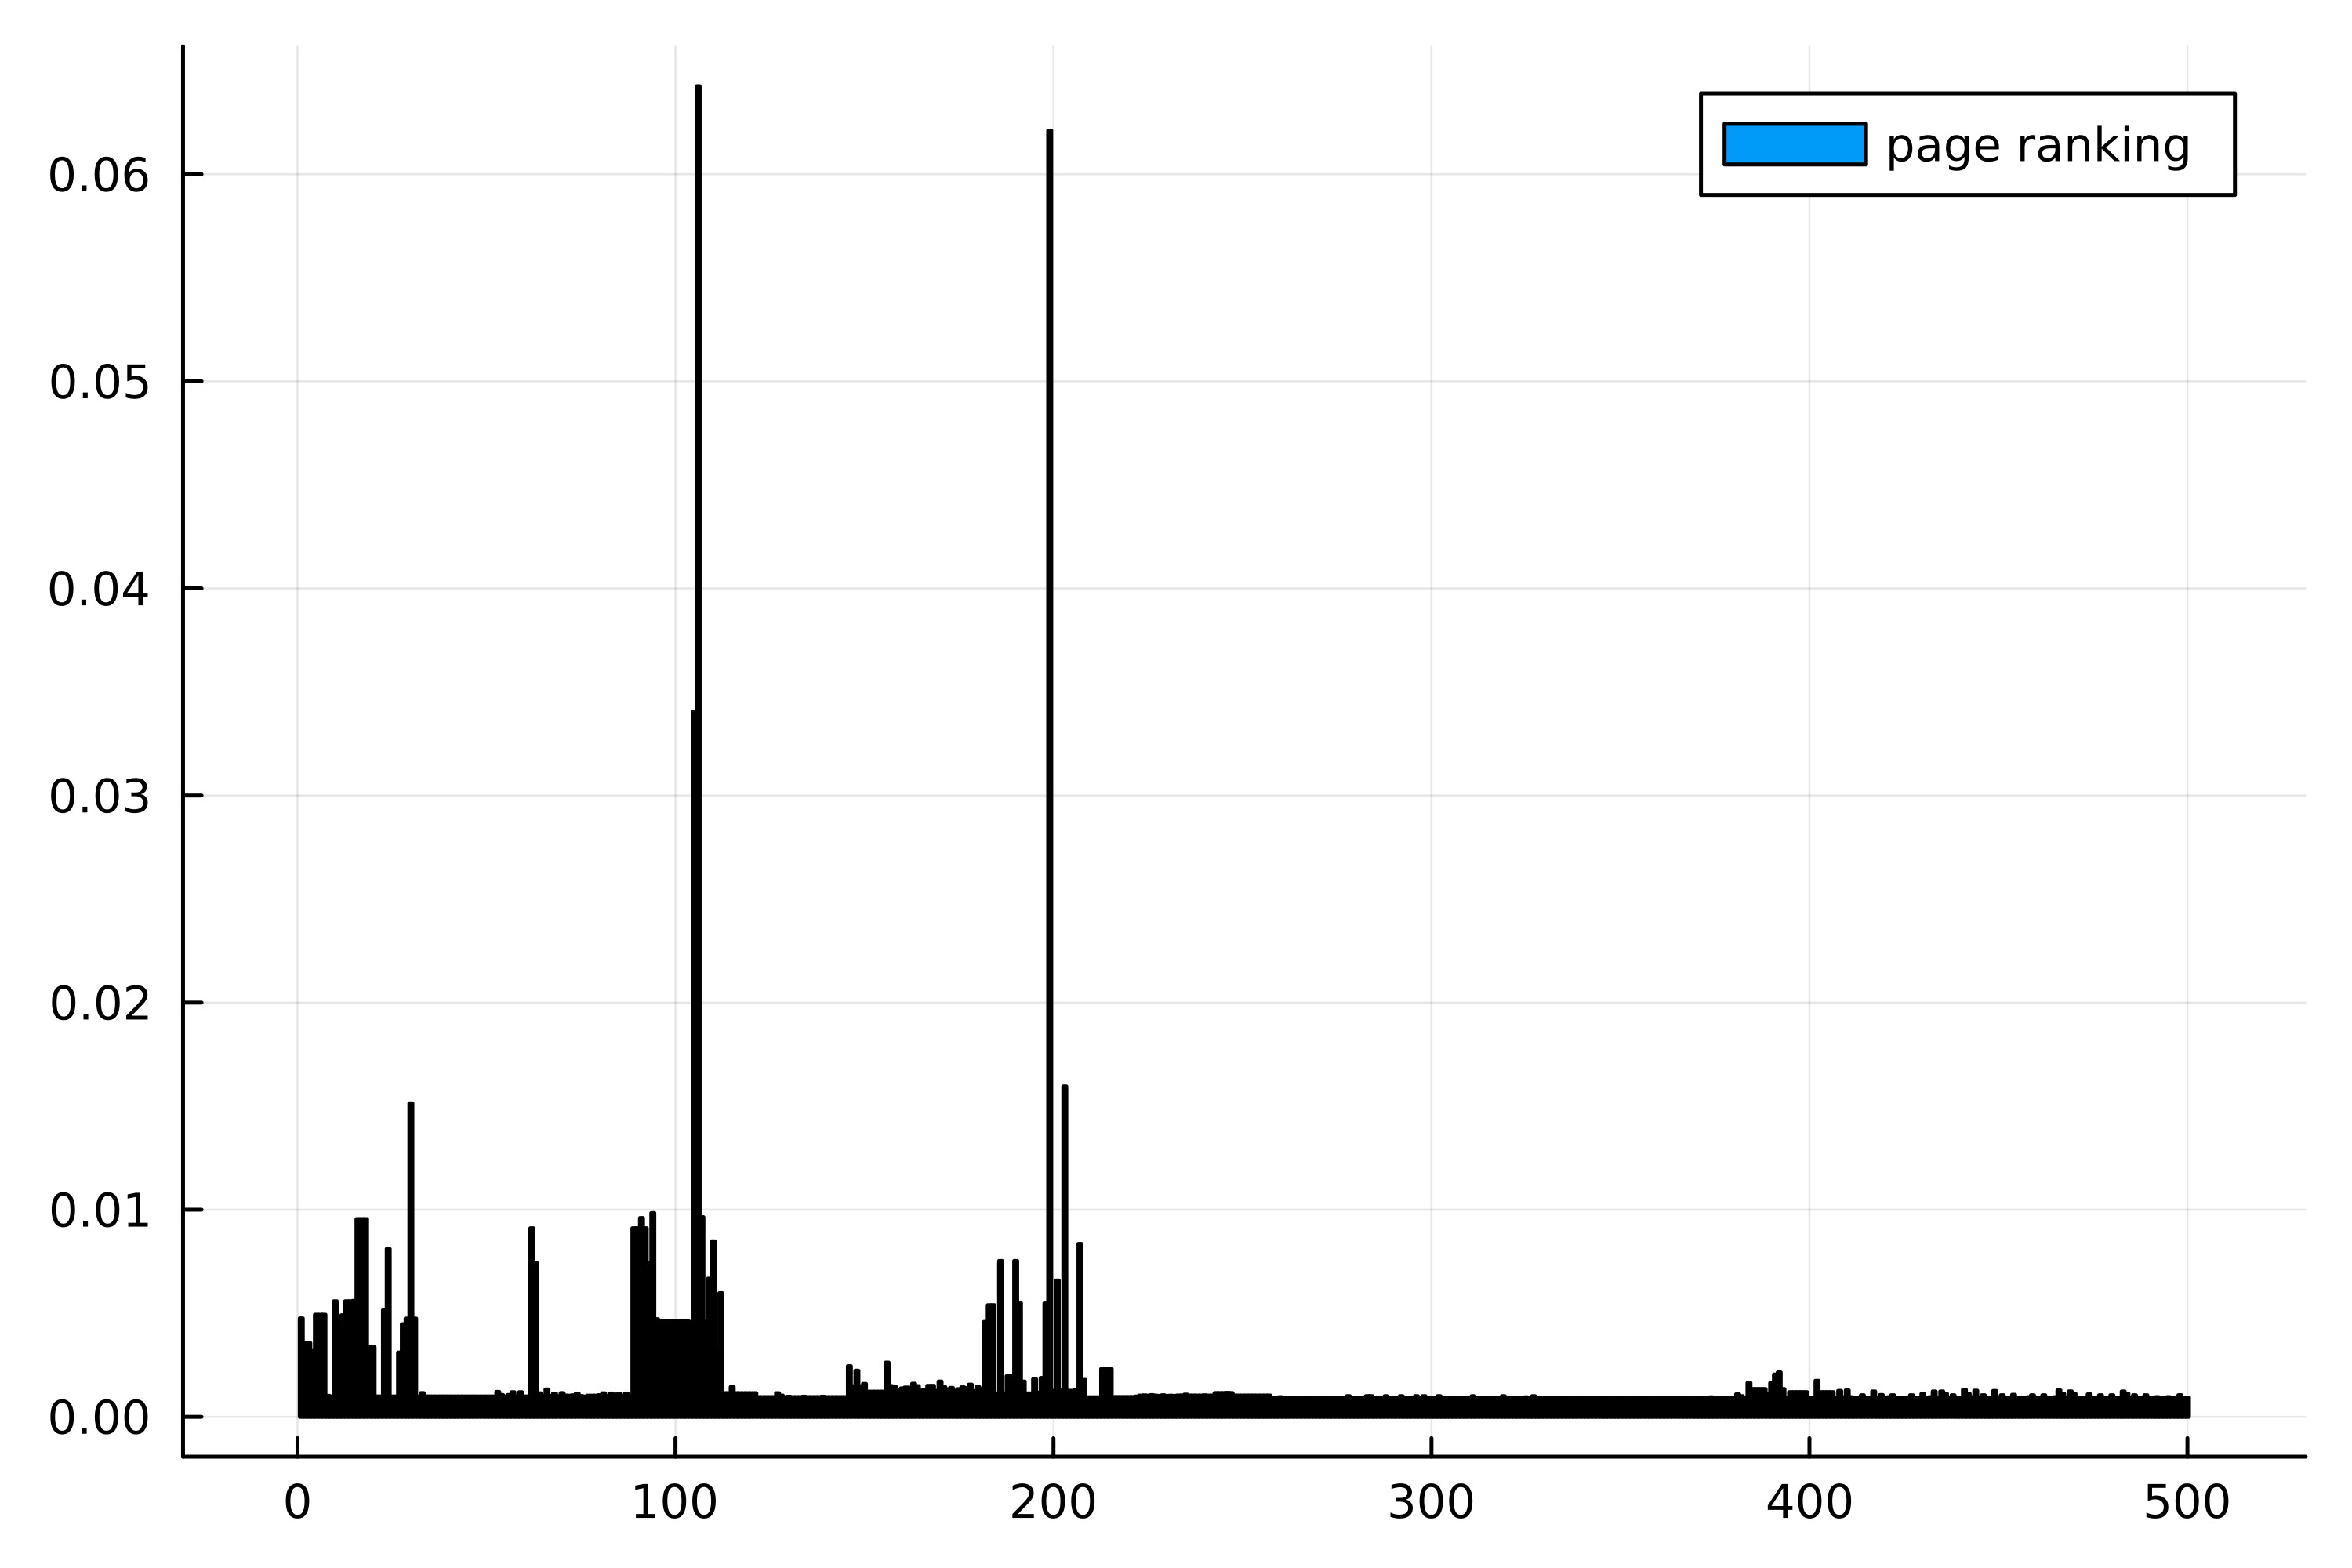
\includegraphics[height=5cm]{fig/StackOverflow_pagerank.jpg}
        \caption{PageRank of chess.com webgraph.}
        \label{fig:StackOverflow_pagerank}
    \end{minipage}
\end{figure}

\begin{table}[!h]
    \small
    \centering
    \begin{tabular}{|l|l|l|l|l|} 
        \hline
        \textbf{Index} & \textbf{Page-rank} & \textbf{In} & \textbf{Out} & \textbf{Url}\\
        \hline
        106 &  0.0642491 & 167 &   1 & \tiny{\url{https://twitter.com/stackoverflow}} \\
        199 &  0.0621094 &  28 &   1 & \tiny{\url{https://www.instagram.com/thestackoverflow/}} \\
        105 &  0.0340524 & 144 &   1 & \tiny{\url{https://www.facebook.com/officialstackoverflow/}} \\
        203 &   0.015951 &   4 &   1 & \tiny{\url{https://talent.stackoverflow.com/users/login}} \\
         30 &  0.0151374 & 183 &  23 & \tiny{\url{https://stackoverflow.co/teams}} \\
         94 &  0.0098377 & 184 &  47 & \tiny{\url{https://stackoverflow.com/legal/cookie-policy}} \\
        107 & 0.00963737 & 166 &   0 & \tiny{\url{https://linkedin.com/company/stack-overflow}} \\
         91 & 0.00959788 & 175 &  47 & \tiny{\url{https://stackoverflow.com/legal/privacy-policy}} \\
         16 & 0.00954374 & 182 &  36 & \tiny{\url{https://stackoverflow.co/}} \\
         17 & 0.00954374 & 182 &  26 & \tiny{\url{https://stackoverflow.co/talent}} \\

        \hline
    \end{tabular}
    \caption{The ten most important entries in the PageRank of the StackOverflow webgraph.}
    \label{table:StackOverflow}
\end{table}

\subsubsection{Conclusions}
As we can see, in every connectivity matrix there are many areas that are not connected to the rest of the webgraph and areas that are very dense.
Matematically speaking, there are many cliques.
This happens because communities or similar links that are really close and they all reference each other, whereas many web pages are not related to each other and therefore are not linked.

Taking the Chess.com connectivity graph as an example (\ref{fig:chesscom}), we can see that the first 60 pages are stlongly connected to each other, 
these are just the different homepages depending on the language of the user (e.g. \url{https://www.chess.com/es}). 
These pages just redirect to the main page and as it can be noticed in the pagerank table \ref{table:chesscom} are even more highly ranked than the main page.


\subsection{Connectivity matrix and subcliques [5 points]}

\subsection{Connectivity matrix and disjoint subgraphs [10 points]}

\subsection{PageRanks by solving a sparse linear system [40 points]}

\subsection{Quality of the Report [15 points]}


\end{document}
